\chapter{Arquitectura del sistema}
\section{Diseño general del sistema}

La aplicación está construida sobre el framework Electron, lo que influencia en gran medida la arquitectura del sistema. Una aplicación en Electron tiene un proceso de ejecución principal que corre Node.js, este se encarga de la comunicación con el sistema operativo, la creación de ventanas, entre otras cosas; utilizando las bibliotecas que provee Electron. El proceso principal a su vez puede crear uno o más procesos renderizadores (renderer process), cada uno con una ventana asignada, estos procesos corren un navegador Chromium que se encarga de desplegar la interfaz de la aplicación (aunque también puede realizar más tareas con scripts de javascript). Esto provoca que la arquitectura este dividida en 2 partes: el proceso principal y el renderer. 

En esta aplicación el renderer es el encargado de desplegar la interfaz de usuario principal donde se  visualizan los documentos pdf y los botones, y demás elementos, usados para las otras funcionalidades del sistema. El proceso principal se encarga de la creación de ventanas del sistema (como la ventana principal, diálogos del sistema, menú contextual, etc), la comunicación con el sistema operativo, las funcionalidades que modifican los documentos y cuenta con el estado de la aplicación.

El código del proyecto tiene un diseño modular basado en los módulos de javascript. En cada módulo se encuentran funciones exportadas (públicas) y las funciones no exportadas (privadas) que solo se utilizan a lo interno del módulo. Cada módulo es responsable de una funcionalidad del sistema. Usualmente un módulo del proceso principal tiene una versión análoga en el renderer.

Para comunicar el proceso principal con el proceso renderer Electron provee la biblioteca IPC (Inter-Process Comunication). En el proyecto la biblioteca se utiliza en el módulo "ipc" que trabaja como una capa de interfaz entre los servicios que provee el proceso principal y el proceso renderer. El proceso renderer se conecta con la interfaz del módulo ipc a través de un preload script que electron carga en el renderer cuando es invocado, este archivo se encuentra en la carpeta raíz del proyecto con el nombre preload.js. 

\subsection{Diagrama de dependencias}

El diagrama de dependencias muestra las dependencias entre los módulos de la aplicación. Es una forma útil de visualizar como trabajan los módulos de la aplicación entre sí y de ver que forma se relacionan. Este diagrama es generado utilizando la herramienta madge, así que muestra el proyecto tal y como está programado. También, puede resultar útil para detectar dependencias circulares o un flujo extraño dentro del programa.

El formato del diagrama es el siguiente. Cada archivo o módulo del sistema es un rectángulo, el color representa el estado de la dependencia: azul si tiene dependencias, verde si no tiene dependencias y rojo si es parte de una dependencia circular. Las flechas indican las dependencias entre módulos.

Hay un diagrama que muestra las dependencias del proceso principal (Ver figura \ref{DiagramaDependenciaMain}) y otro que muestra el proceso renderer (Ver figura \ref{DiagramaDependenciaRenderer}).

\subsubsection{Proceso principal}

\begin{figure}[H]
	\centering
	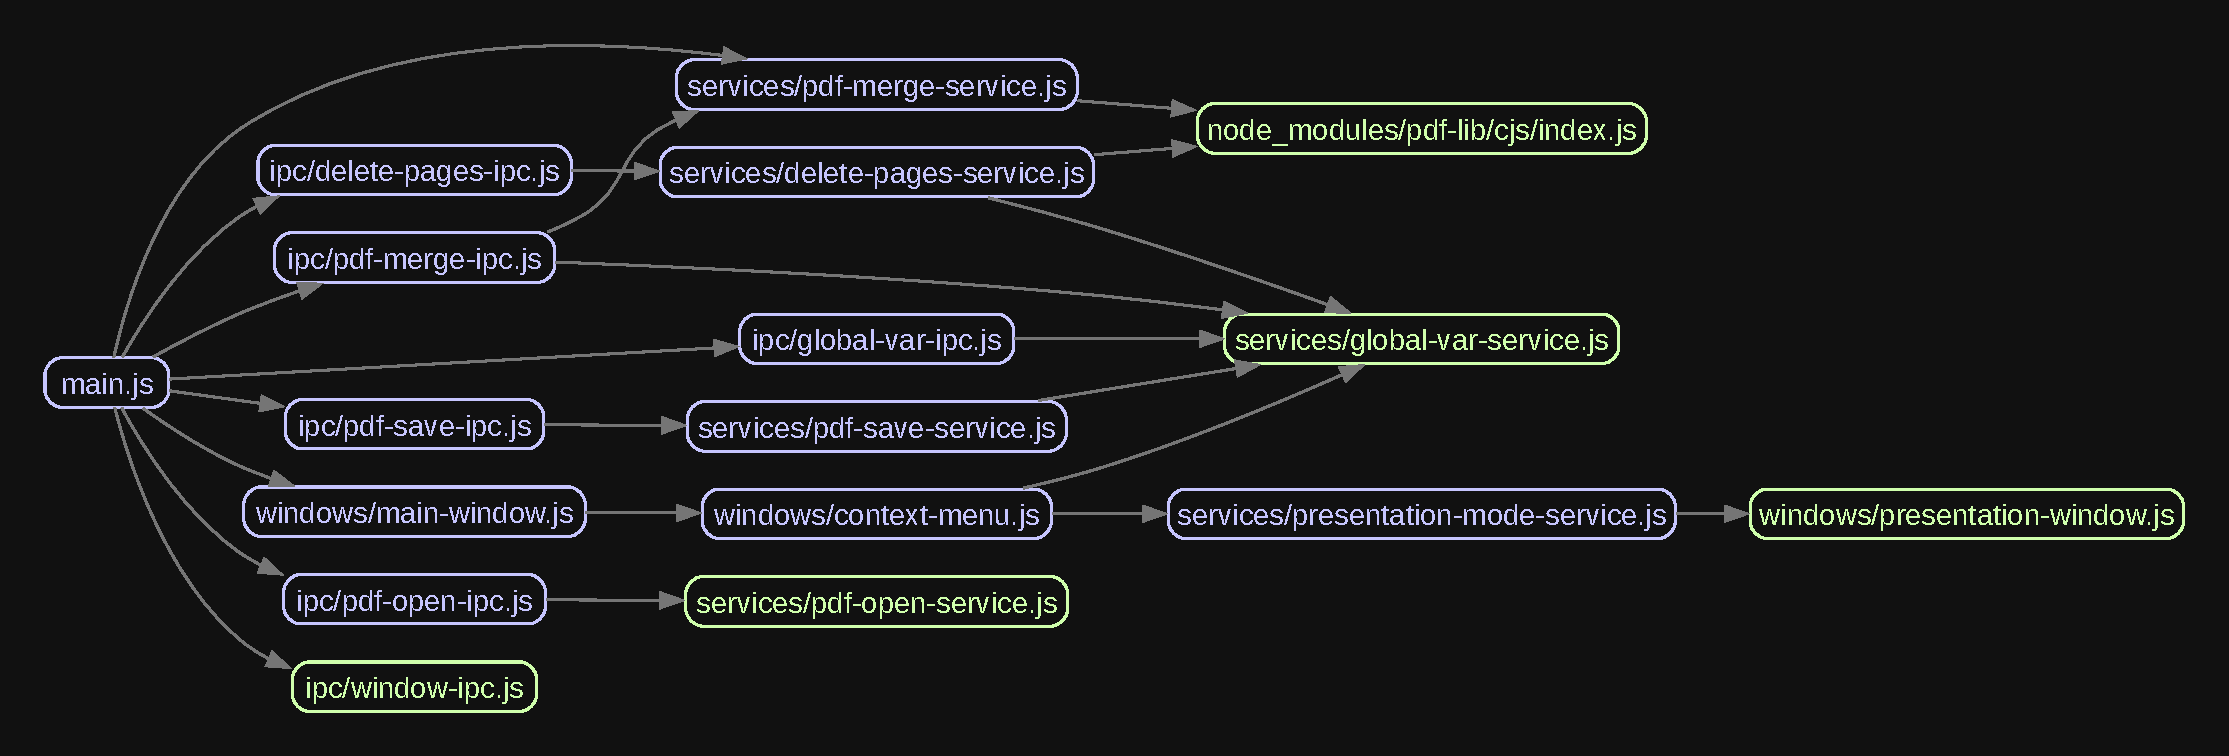
\includegraphics[width=\linewidth]{project/images/dd_main.pdf}
	\caption{\textbf{Diagrama de Dependencias: proceso principal}}
	\label{DiagramaDependenciaMain}
\end{figure}

\subsubsection{Proceso renderer}

\begin{figure}[H]
	\centering
	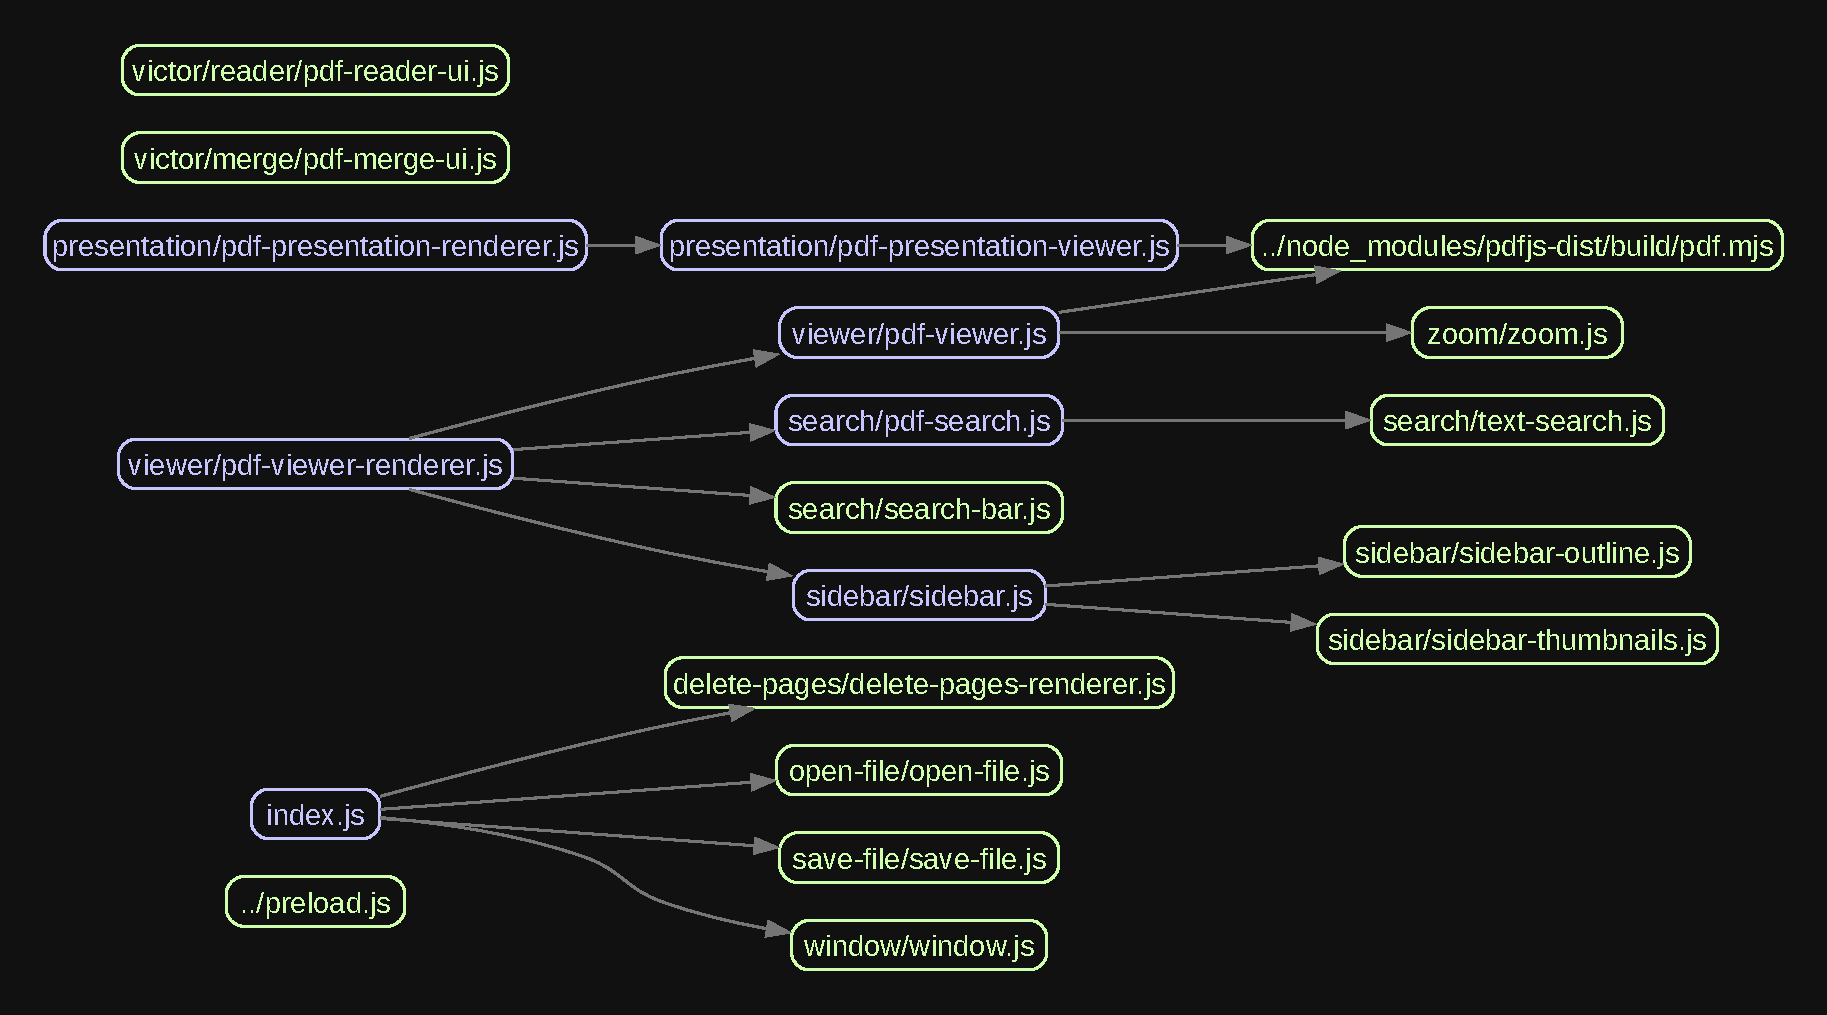
\includegraphics[width=\linewidth]{project/images/dd_renderer.pdf}
	\caption{\textbf{Diagrama de Dependencias: proceso renderer}}
	\label{DiagramaDependenciaRenderer}
\end{figure}


\subsection{Diagrama de bloques}

El diagrama de bloques muestra la organización de los módulos del proyecto y cómo se comunican entre sí de forma superficial. Este diagrama es útil para entender la estructura del proyecto ya que la jerarquía de módulos es similar a la estructura de archivos que tiene el proyecto. 

El diagrama (Ver figura \ref{DiagramaBloques}) expone 2 bloques principales: proceso principal y renderer. El bloque del proceso principal tiene el módulo "windows" que tiene ventanas del sistema, el módulo "services" que tiene módulos con funcionalidades del programa y el módulo "ipc" que expone módulos del proceso principal al proceso renderer. El bloque del proceso renderer tiene 2 módulos: index y presentation, cada corresponde a una página de la interfaz de la aplicación.

\begin{figure}[H]
	\centering
	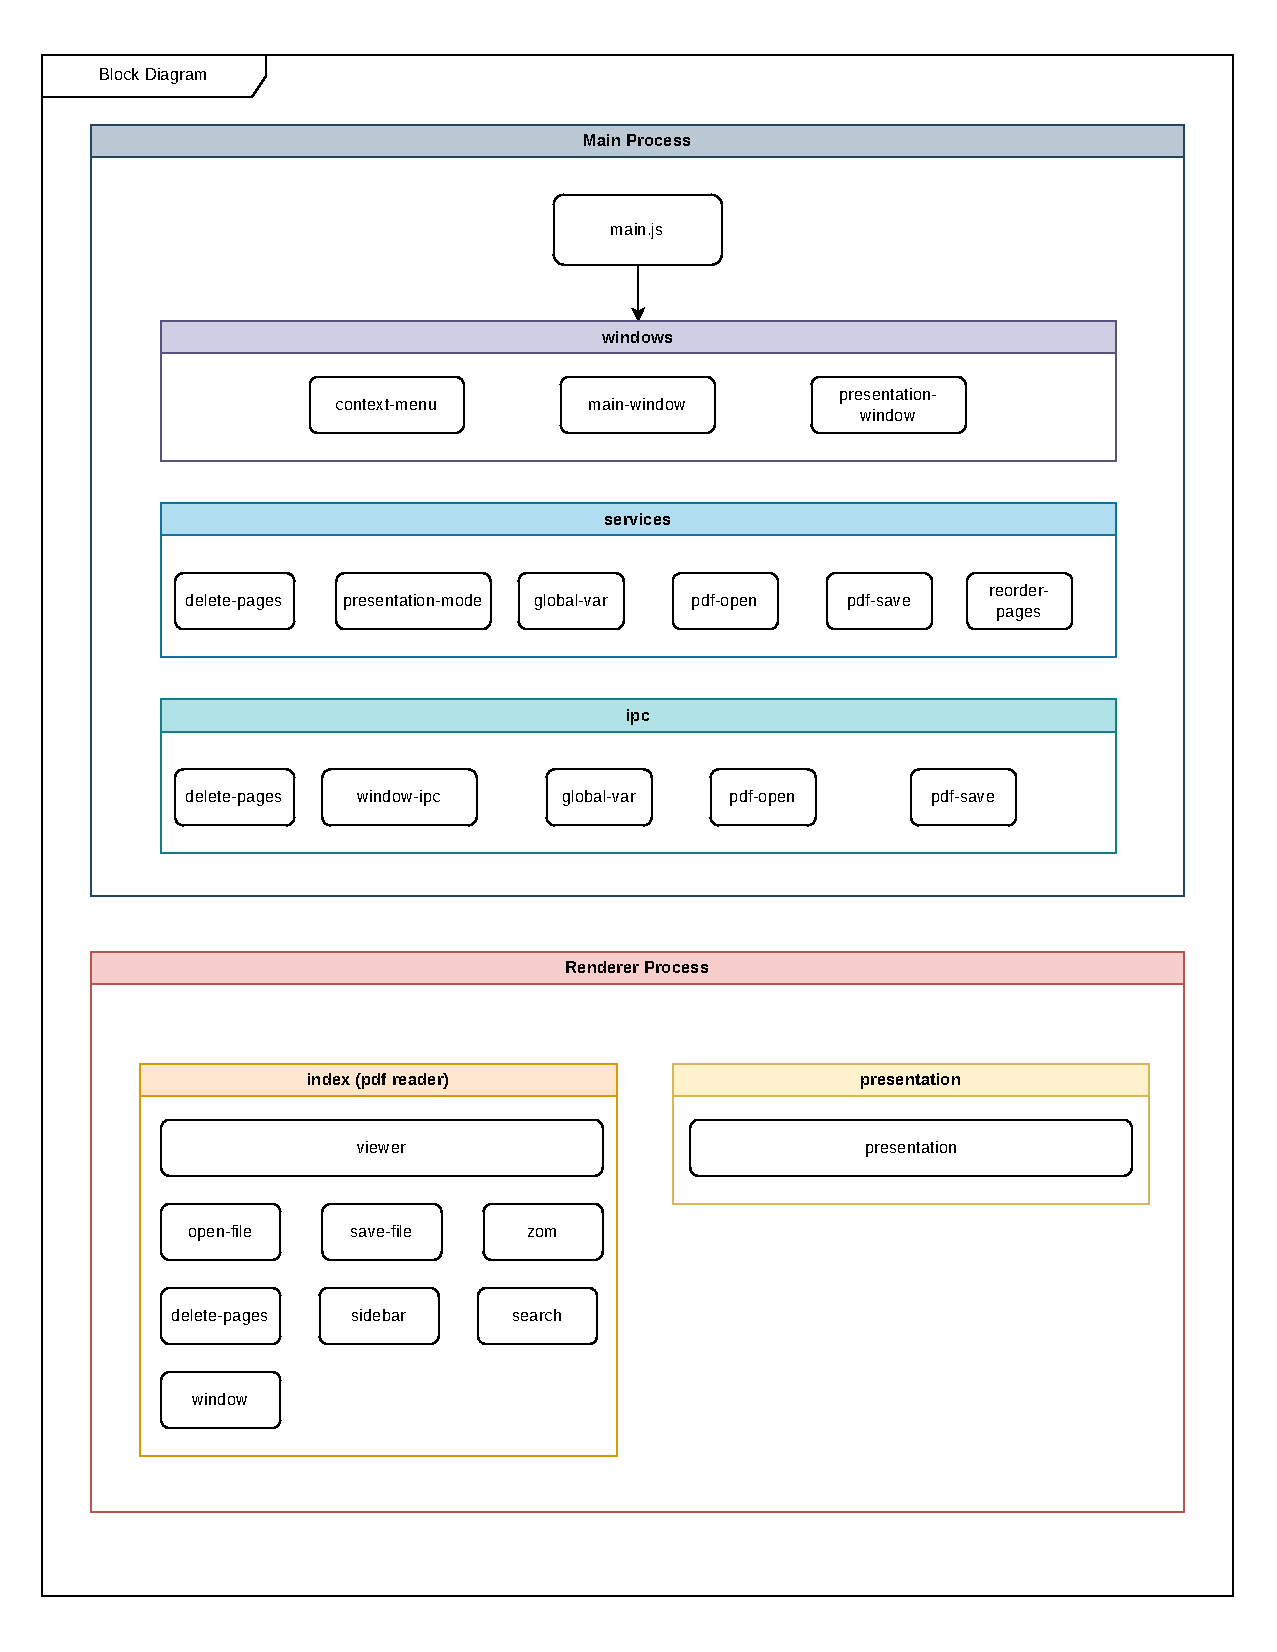
\includegraphics[width=\linewidth]{project/images/BlockDiagram.pdf}
	\caption{\textbf{Diagrama de Bloques}}
	\label{DiagramaBloques}
\end{figure}

\subsection{Diagrama de Clases}

El diagrama de clases describe las clases que existen dentro de la aplicación. El diagrama (Ver figura \ref{DiagramaClases}) muestra 2 clases. La clase PdfViewer es la encargada de mostrar el pdf dentro de la aplicación, además muestra información como número de página actual y tiene herramientas como el zoom. La clase PresentationViewer se encarga de mostrar el pdf en modo presentación.

\begin{figure}[H]
	\centering
	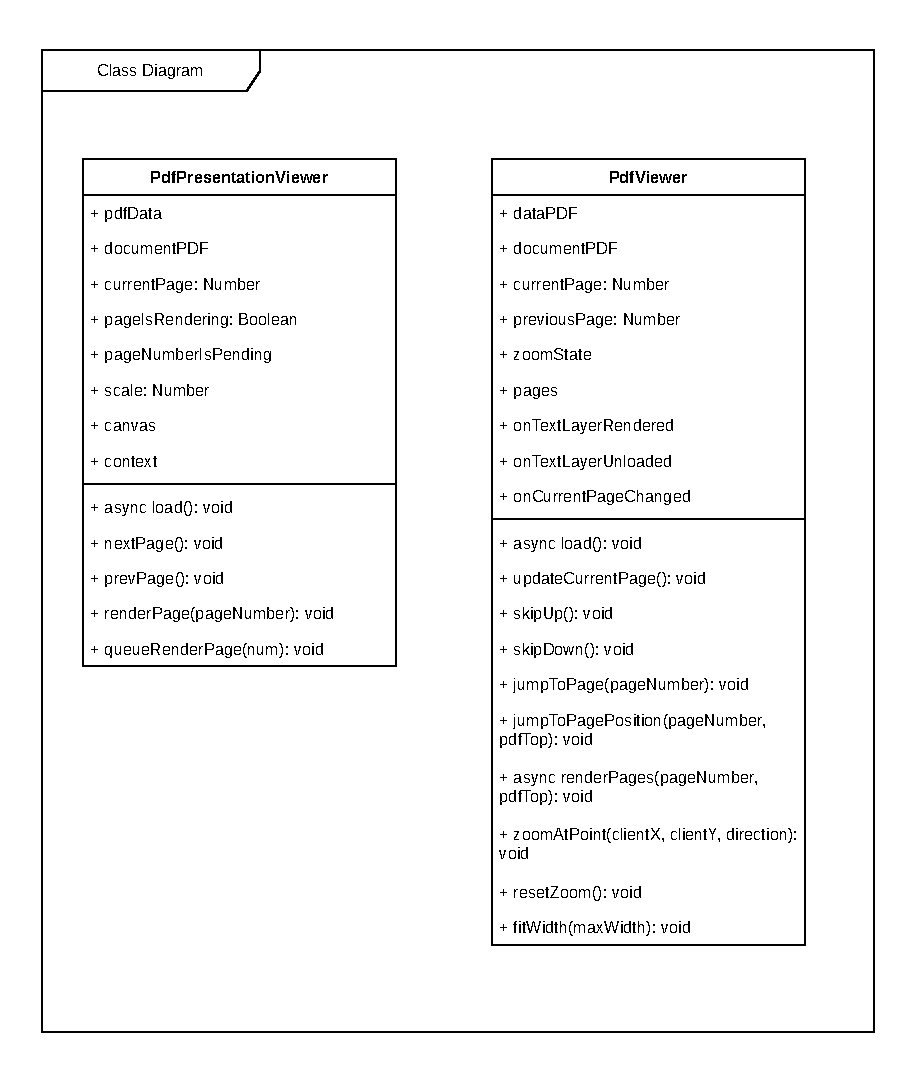
\includegraphics[width=\linewidth]{project/images/ClassDiagram.pdf}
	\caption{\textbf{Diagrama de Clases}}
	\label{DiagramaClases}
\end{figure}



